\documentclass[aspectratio=169,10pt]{beamer}

\usepackage{amsmath,amssymb,booktabs,graphicx,microtype}
\usepackage{tikz}
\usetikzlibrary{arrows.meta,positioning,calc,fit}

% Restrained physics-talk palette.
\definecolor{navy}{RGB}{19,55,91}
\definecolor{blue}{RGB}{40,112,164}
\definecolor{sky}{RGB}{222,237,247}
\definecolor{orange}{RGB}{225,112,32}
\definecolor{gold}{RGB}{246,190,74}
\definecolor{green}{RGB}{47,126,82}
\definecolor{red}{RGB}{174,54,48}
\definecolor{ink}{RGB}{35,40,46}
\definecolor{muted}{RGB}{100,108,117}
\definecolor{paper}{RGB}{249,250,252}

\setbeamercolor{normal text}{fg=ink,bg=white}
\setbeamercolor{structure}{fg=navy}
\setbeamercolor{frametitle}{fg=white,bg=navy}
\setbeamercolor{title}{fg=white}
\setbeamercolor{subtitle}{fg=sky}
\setbeamercolor{author}{fg=white}
\setbeamercolor{institute}{fg=sky}
\setbeamercolor{date}{fg=sky}
\setbeamercolor{block title}{fg=white,bg=navy}
\setbeamercolor{block body}{fg=ink,bg=paper}
\setbeamercolor{alerted text}{fg=red}

\setbeamertemplate{navigation symbols}{}
\setbeamertemplate{itemize item}{\color{blue}$\blacktriangleright$}
\setbeamertemplate{itemize subitem}{\color{orange}$\bullet$}
\setbeamertemplate{frametitle}{%
  \nointerlineskip
  \begin{beamercolorbox}[wd=\paperwidth,ht=0.72cm,dp=0.24cm,leftskip=0.52cm]{frametitle}
    \usebeamerfont{frametitle}\insertframetitle
  \end{beamercolorbox}}
\setbeamertemplate{footline}{%
  \leavevmode
  \hbox{%
    \begin{beamercolorbox}[wd=.82\paperwidth,ht=2.6ex,dp=1.1ex,leftskip=.5cm]{author in head/foot}%
      \color{muted}\scriptsize Neural posterior extraction of GPDs
    \end{beamercolorbox}%
    \begin{beamercolorbox}[wd=.18\paperwidth,ht=2.6ex,dp=1.1ex,rightskip=.45cm plus1fil]{date in head/foot}%
      \color{muted}\scriptsize\insertframenumber/15
    \end{beamercolorbox}}
  \vskip0pt}

\setbeamersize{text margin left=0.55cm,text margin right=0.55cm}
\graphicspath{{assets/current_plots/}{assets/}}

\newcommand{\Huplus}{H_u^{+}}
\newcommand{\Huminus}{H_u^{-}}
\newcommand{\takeaway}[1]{%
  \vspace{1mm}\begin{beamercolorbox}[rounded=true,sep=1.4mm,wd=\linewidth]{block body}%
  \centering\color{navy}\bfseries #1
  \end{beamercolorbox}}
\newcommand{\galleryplot}[1]{%
  \centering
  \includegraphics[width=.94\linewidth,height=.77\textheight,keepaspectratio]{#1}}
\newcommand{\holdoutplot}[1]{%
  \centering
  \includegraphics[width=.92\linewidth,height=.78\textheight,keepaspectratio]
    {holdout_plots/holdout-#1.png}}

\tikzset{
  flow/.style={-Latex,very thick,draw=navy},
  box/.style={rounded corners=2pt,draw=navy,very thick,fill=sky,
              align=center,minimum height=1.05cm,text width=2.55cm},
  warmbox/.style={box,draw=orange,fill=orange!10},
  greenbox/.style={box,draw=green,fill=green!10},
  badbox/.style={box,draw=red,fill=red!7}
}

\title{Inferring generalized parton distributions from DVCS observables}
\subtitle{A neural posterior solution to an ill-posed inverse problem\\[1mm]
Full-sector synthetic closure and native-model holdout tests}
\author{Avnish Singh}
\institute{Jefferson Lab Hall C / NPS analysis}
\date{31 August 2026}

\begin{document}

\begin{frame}[plain]
  \begin{tikzpicture}[remember picture,overlay]
    \fill[navy] (current page.south west) rectangle (current page.north east);
    \fill[blue!35!navy] (current page.south west) rectangle
      ([xshift=3.0cm]current page.north west);
    \draw[orange,line width=3pt]
      ([xshift=3.0cm]current page.south west) --
      ([xshift=3.0cm]current page.north west);
  \end{tikzpicture}
  \vspace{1.35cm}
  \hspace{2.9cm}\begin{minipage}{0.73\textwidth}
    {\color{white}\LARGE\bfseries\inserttitle\par}
    \vspace{0.45cm}
    {\color{sky}\large\insertsubtitle\par}
    \vspace{1.05cm}
    {\color{white}\insertauthor\par}
    {\color{sky}\small\insertinstitute\par}
    \vspace{0.25cm}
    {\color{sky}\small\insertdate\par}
  \end{minipage}
\end{frame}

\begin{frame}{The target is a posterior over the full modeled GPD content}
\begin{columns}[T,onlytextwidth]
\column{0.52\textwidth}
Generalized parton distributions connect longitudinal momentum and transverse
spatial structure while retaining the amplitude-level information probed by
exclusive scattering. The learned object is
\[
 q_\varphi(\theta,\eta\mid D),
 \qquad \dim(\theta,\eta)=80+2,
\]
with independent modeled sectors
\[
 F\in\{H,E,\widetilde H,\widetilde E\},
 \qquad p\in\{u,d,s,g\}.
\]
Posterior samples define the corresponding GPD curves and, after exact PARTONS
reevaluation, CFFs and observables.

\column{0.45\textwidth}
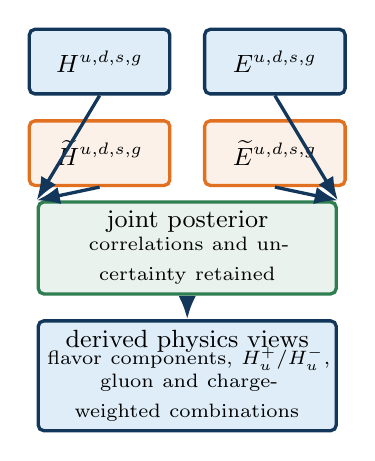
\begin{tikzpicture}[node distance=3mm and 4mm,font=\small]
  \node[box,text width=1.55cm,minimum height=.82cm] (h) {$H^{u,d,s,g}$};
  \node[box,text width=1.55cm,minimum height=.82cm,right=of h] (e) {$E^{u,d,s,g}$};
  \node[warmbox,text width=1.55cm,minimum height=.82cm,below=of h] (ht) {$\widetilde H^{u,d,s,g}$};
  \node[warmbox,text width=1.55cm,minimum height=.82cm,right=of ht] (et) {$\widetilde E^{u,d,s,g}$};
  \node[greenbox,text width=3.55cm,minimum height=.92cm,
    below=6mm of $(ht)!0.5!(et)$] (post)
    {joint posterior\\[-1mm]\scriptsize correlations and uncertainty retained};
  \node[box,text width=3.55cm,minimum height=1.15cm,below=of post] (derived)
    {derived physics views\\[-1mm]\scriptsize flavor components, $\Huplus/\Huminus$,\\[-1mm]
     \scriptsize gluon and charge-weighted combinations};
  \draw[flow] (h.south) -- (post.north west);
  \draw[flow] (e.south) -- (post.north east);
  \draw[flow] (ht.south) -- (post.north west);
  \draw[flow] (et.south) -- (post.north east);
  \draw[flow] (post) -- (derived);
\end{tikzpicture}
\end{columns}
\takeaway{$\Huplus$ and $\Huminus$ are representative derived components---not the unique or primary network output.}
\end{frame}

\begin{frame}{DVCS constrains convolutions, not pointwise GPD values}
\begin{columns}[T,onlytextwidth]
\column{0.57\textwidth}
At each measured $(x_B,t,Q^2,\phi)$, the native calculation performs
\[
\begin{aligned}
F(x,\xi,t,Q_0^2)&\xrightarrow{\mathrm{QCD\ evolution}}
F(x,\xi,t,Q^2),\\[-1mm]
\mathcal F(\xi,t,Q^2)&=\int_{-1}^{1}dx\;C(x,\xi,Q^2)F(x,\xi,t,Q^2),
\end{aligned}
\]
where $\mathcal F\in\{\mathcal H,\mathcal E,
\widetilde{\mathcal H},\widetilde{\mathcal E}\}$ is a complex Compton form
factor (CFF).

\vspace{2mm}
The measured quantity is then built from
\[
  |T_{\rm BH}+T_{\rm DVCS}|^2
  =|T_{\rm BH}|^2+2\Re(T_{\rm BH}T_{\rm DVCS}^{*})+|T_{\rm DVCS}|^2.
\]

\column{0.40\textwidth}
\begin{block}{Six complementary observables}
\small
\begin{itemize}\setlength\itemsep{2mm}
  \item unpolarized / beam-spin half-sum
  \item beam-spin difference
  \item beam-charge asymmetry
  \item beam-spin asymmetry
  \item longitudinal target-spin asymmetry
  \item longitudinal double-spin asymmetry
\end{itemize}
\end{block}
\end{columns}
\takeaway{Different observables probe different CFF combinations, but none is a direct measurement of $H^u(x,\xi,t)$.}
\end{frame}

\begin{frame}{The observable does not uniquely determine the underlying GPD}
\centering
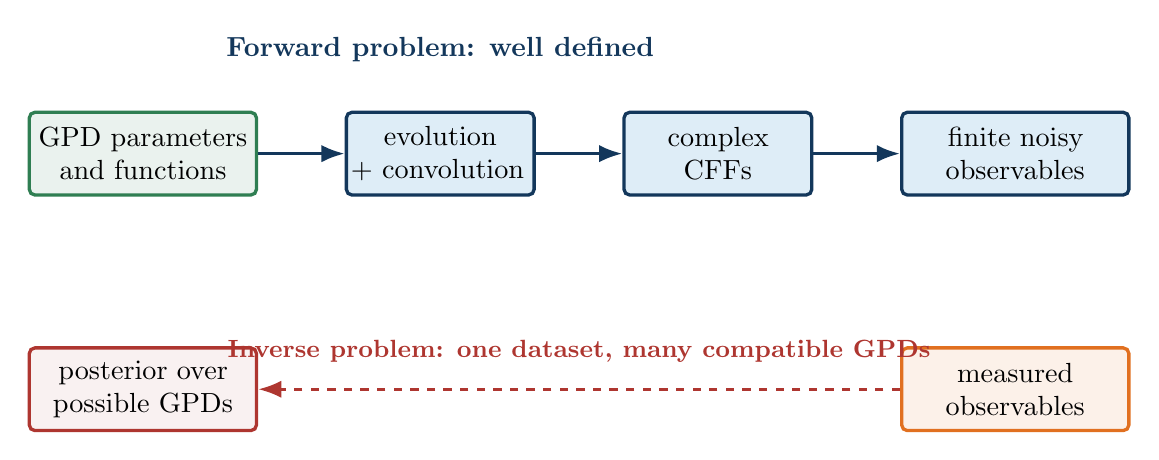
\begin{tikzpicture}[node distance=7mm and 11mm]
  \node[greenbox,text width=2.65cm] (gpd) {GPD parameters\\and functions};
  \node[box,right=of gpd,text width=2.15cm] (evo) {evolution\\+ convolution};
  \node[box,right=of evo,text width=2.15cm] (cff) {complex\\CFFs};
  \node[box,right=of cff,text width=2.65cm] (obs) {finite noisy\\observables};
  \draw[flow] (gpd) -- (evo);
  \draw[flow] (evo) -- (cff);
  \draw[flow] (cff) -- (obs);
  \node[above=5mm of evo,navy,font=\bfseries] {Forward problem: well defined};

  \node[badbox,text width=2.65cm,below=19mm of gpd] (igpd)
    {posterior over\\possible GPDs};
  \node[warmbox,text width=2.65cm,below=19mm of obs] (iobs)
    {measured\\observables};
  \draw[-Latex,very thick,draw=red,dashed] (iobs) -- node[above=2mm,align=center,
    text=red,font=\small\bfseries] {Inverse problem: one dataset, many compatible GPDs} (igpd);
\end{tikzpicture}

\vspace{4mm}
\begin{columns}[T,onlytextwidth]
\column{0.32\textwidth}\centering
\textbf{Information is compressed}\\[-1mm]
\small CFF convolution integrates over $x$.
\column{0.32\textwidth}\centering
\textbf{Directions are degenerate}\\[-1mm]
\small Correlated GPD changes can leave observables nearly unchanged.
\column{0.32\textwidth}\centering
\textbf{Coverage is finite}\\[-1mm]
\small Limited kinematics and uncertainty amplify ambiguity.
\end{columns}
\end{frame}

\begin{frame}{We learn a posterior inverse map, not a pointwise inverse}
\begin{columns}[T,onlytextwidth]
\column{0.57\textwidth}
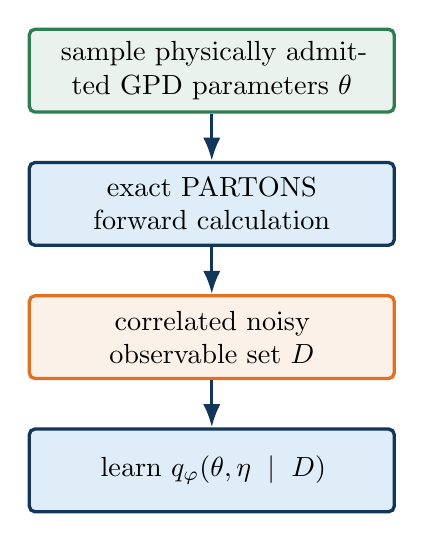
\begin{tikzpicture}[node distance=6mm]
  \node[greenbox,text width=4.4cm] (prior)
    {sample physically admitted GPD parameters $\theta$};
  \node[box,text width=4.4cm,below=of prior] (forward)
    {exact PARTONS forward calculation};
  \node[warmbox,text width=4.4cm,below=of forward] (data)
    {correlated noisy observable set $D$};
  \node[box,text width=4.4cm,below=of data] (learn)
    {learn $q_\varphi(\theta,\eta\mid D)$};
  \draw[flow] (prior)--(forward);
  \draw[flow] (forward)--(data);
  \draw[flow] (data)--(learn);
\end{tikzpicture}

\column{0.40\textwidth}
\vspace{5mm}
\[
\mathcal L_{\rm NPE}
=-\mathbb E_{\theta,D}\!\left[
  \log q_\varphi(\theta,\eta\mid D)
\right].
\]
\small
The network learns which regions of the declared physics parameter space are
compatible with an unordered set of observables. Posterior samples are then
reevaluated through the exact native calculation to obtain CFF and GPD bands.

\vspace{3mm}
\textcolor{red}{No uniqueness is imposed: weakly identified directions should
remain broad.}
\end{columns}
\end{frame}

\begin{frame}{Physics information is compressed before posterior inference}
\centering
\resizebox{.95\linewidth}{!}{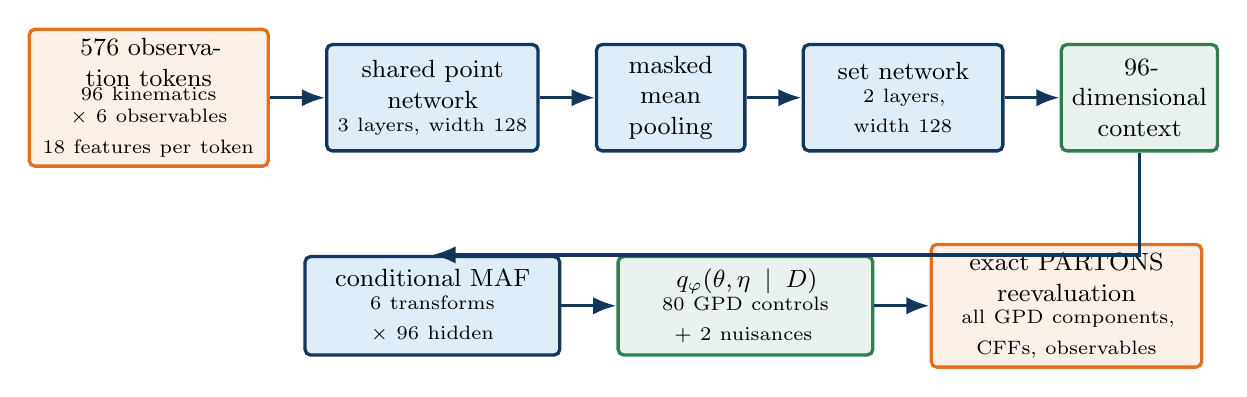
\begin{tikzpicture}[node distance=5mm and 7mm,font=\small]
  \node[warmbox,text width=2.8cm,minimum height=1.35cm] (tokens)
    {576 observation tokens\\[-1mm]
     \scriptsize 96 kinematics $\times$ 6 observables\\
     \scriptsize 18 features per token};
  \node[box,right=of tokens,text width=2.45cm,minimum height=1.35cm] (point)
    {shared point network\\[-1mm]
     \scriptsize 3 layers, width 128};
  \node[box,right=of point,text width=1.65cm,minimum height=1.35cm] (pool)
    {masked mean\\pooling};
  \node[box,right=of pool,text width=2.3cm,minimum height=1.35cm] (set)
    {set network\\[-1mm]
     \scriptsize 2 layers, width 128};
  \node[greenbox,right=of set,text width=1.75cm,minimum height=1.35cm] (embed)
    {96-dimensional\\context};
  \draw[flow] (tokens)--(point);
  \draw[flow] (point)--(pool);
  \draw[flow] (pool)--(set);
  \draw[flow] (set)--(embed);

  \node[box,text width=3.0cm,minimum height=1.25cm,below=13mm of point] (maf)
    {conditional MAF\\[-1mm]
     \scriptsize 6 transforms $\times$ 96 hidden};
  \node[greenbox,text width=3.0cm,minimum height=1.25cm,right=of maf] (post)
    {$q_\varphi(\theta,\eta\mid D)$\\[-1mm]
     \scriptsize 80 GPD controls + 2 nuisances};
  \node[warmbox,text width=3.2cm,minimum height=1.25cm,right=of post] (curves)
    {exact PARTONS reevaluation\\[-1mm]
     \scriptsize all GPD components, CFFs, observables};
  \draw[flow] (embed.south) |- (maf.north);
  \draw[flow] (maf)--(post);
  \draw[flow] (post)--(curves);
\end{tikzpicture}}

\vspace{4mm}
\small Each token contains kinematics, observable identity, normalized value,
uncertainty, full-covariance whitening information, nuisance responses, and a mask.
Permutation-invariant pooling makes the inference depend on the dataset, not its ordering.
\end{frame}

\begin{frame}{The training corpus is generated from a broad physics model space}
\begin{columns}[T,onlytextwidth]
\column{0.56\textwidth}
\footnotesize
At $Q_0^2=1\,\mathrm{GeV}^2$, each of
$F\in\{H,E,\widetilde H,\widetilde E\}$ and
$p\in\{u,d,s,g\}$ has an independent double-distribution block:
\[
F^p=\int d\beta\,d\alpha\,
\delta(x-\beta-\xi\alpha)\,
f_{F,p}(\beta,t)\,\pi_{b_{F,p}}(\beta,\alpha),
\]
\[
f_{F,p}\propto
N_{F,p}\,\beta^{a_{F,p}}(1-\beta)^{c_{F,p}}e^{B_{F,p}t}.
\]
Five controls $(N,a,c,b,B)$ for each of 16 blocks give
\textbf{80 independent physics coordinates}.

\vspace{1mm}
Declared support includes $N\in(-4,4)$, $a\in(0.1,1)$,
$c\in(2,6)$, $b\in(1,4)$, and $B\in(0,2)\,\mathrm{GeV}^{-2}$.

\column{0.41\textwidth}
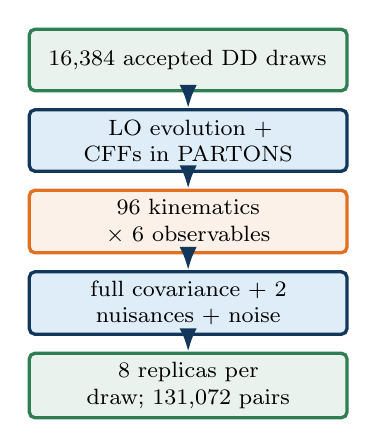
\begin{tikzpicture}[node distance=2mm,font=\footnotesize]
  \node[greenbox,text width=3.8cm,minimum height=.78cm] (m) {16,384 accepted DD draws};
  \node[box,text width=3.8cm,minimum height=.78cm,below=of m] (p) {LO evolution + CFFs in PARTONS};
  \node[warmbox,text width=3.8cm,minimum height=.78cm,below=of p] (o) {96 kinematics $\times$ 6 observables};
  \node[box,text width=3.8cm,minimum height=.78cm,below=of o] (n) {full covariance + 2 nuisances + noise};
  \node[greenbox,text width=3.8cm,minimum height=.78cm,below=of n] (pairs) {8 replicas per draw; 131,072 pairs};
  \draw[flow] (m)--(p); \draw[flow] (p)--(o);
  \draw[flow] (o)--(n); \draw[flow] (n)--(pairs);
\end{tikzpicture}
\end{columns}
\takeaway{The corpus spans a declared DD-induced solution space; it is broad, but not model independent.}
\end{frame}

\begin{frame}{Grouped splits prevent noisy replicas from leaking across roles}
\begin{columns}[T,onlytextwidth]
\column{0.44\textwidth}
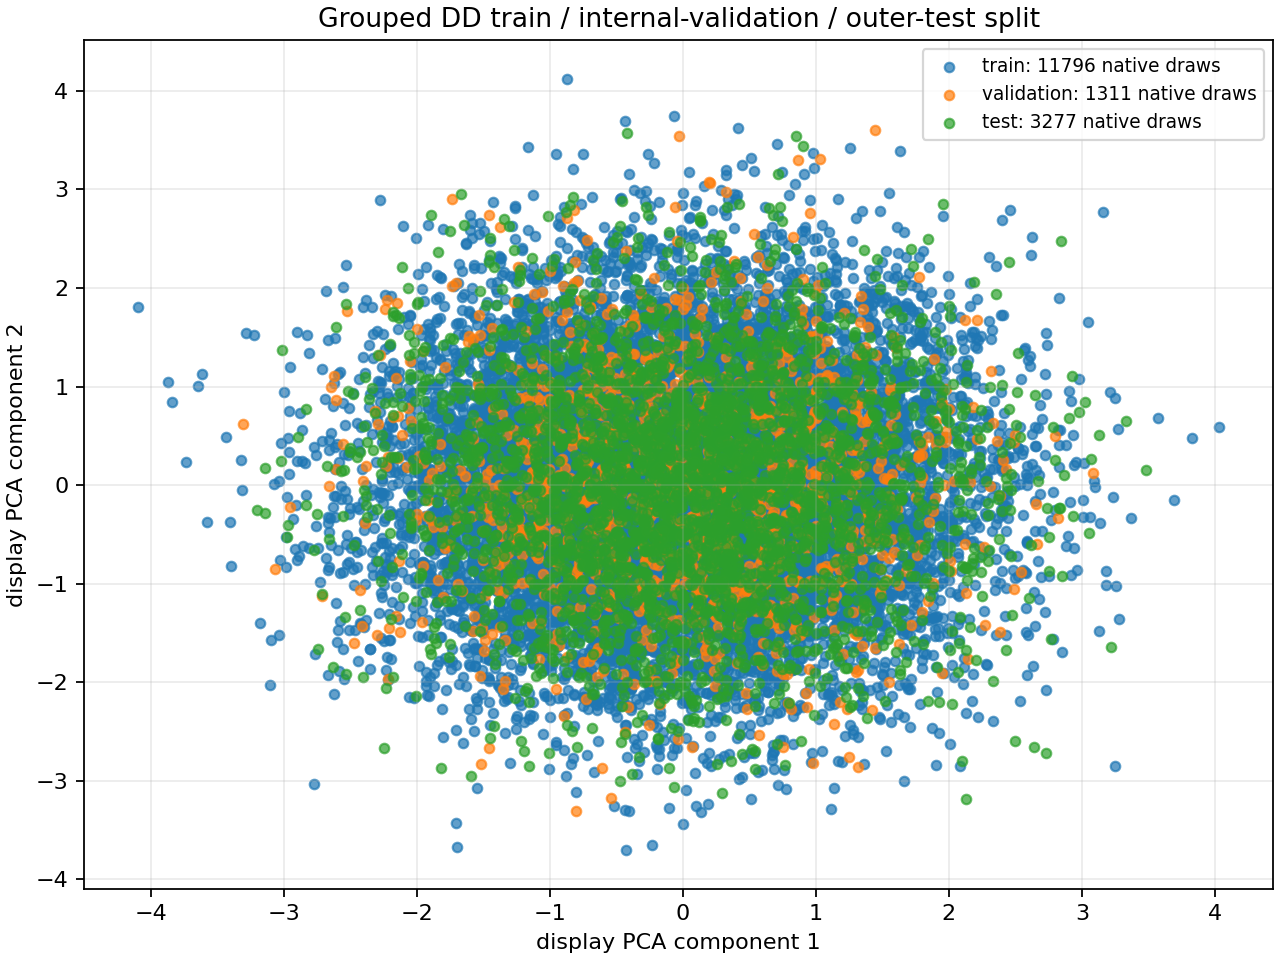
\includegraphics[width=\linewidth,height=.56\textheight,keepaspectratio]{dd_train_validation_test_split.png}
\column{0.53\textwidth}
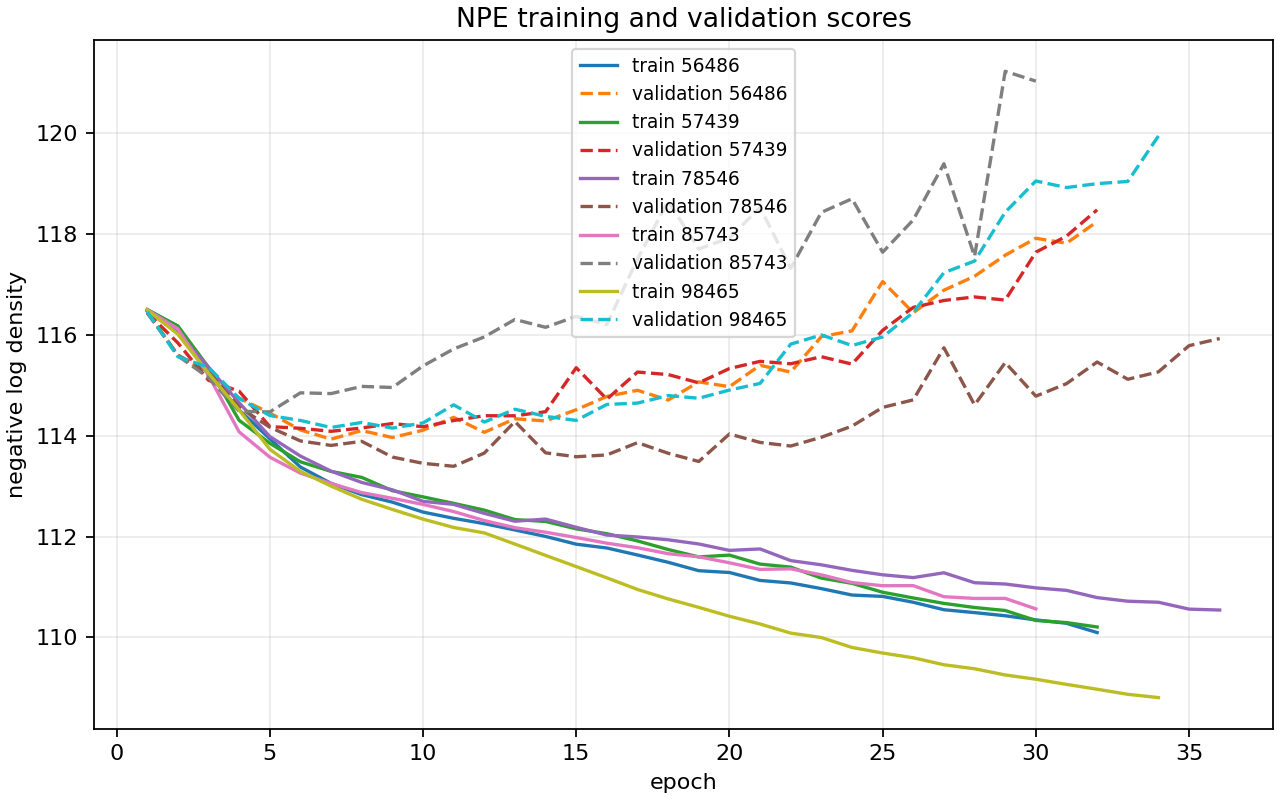
\includegraphics[width=\linewidth,height=.40\textheight,keepaspectratio]{training_validation_nll.png}
\vspace{-1mm}
\begin{itemize}\scriptsize\setlength\itemsep{.7mm}
  \item 11,796 train / 1,311 internal validation / 3,277 locked outer-test parameter groups.
  \item Replicas from one physics draw remain in the same role.
  \item Validation NLL turns upward after its minimum: later epochs overfit.
  \item Early stopping selects the validation minimum; the outer test is never used for training or member selection.
\end{itemize}
\end{columns}
\takeaway{Selected ensemble: mean train NLL 112.76, mean outer-test NLL 113.91; worst test--validation gap 0.112.}
\end{frame}

\begin{frame}{Repeated synthetic closure is consistent with calibrated uncertainty}
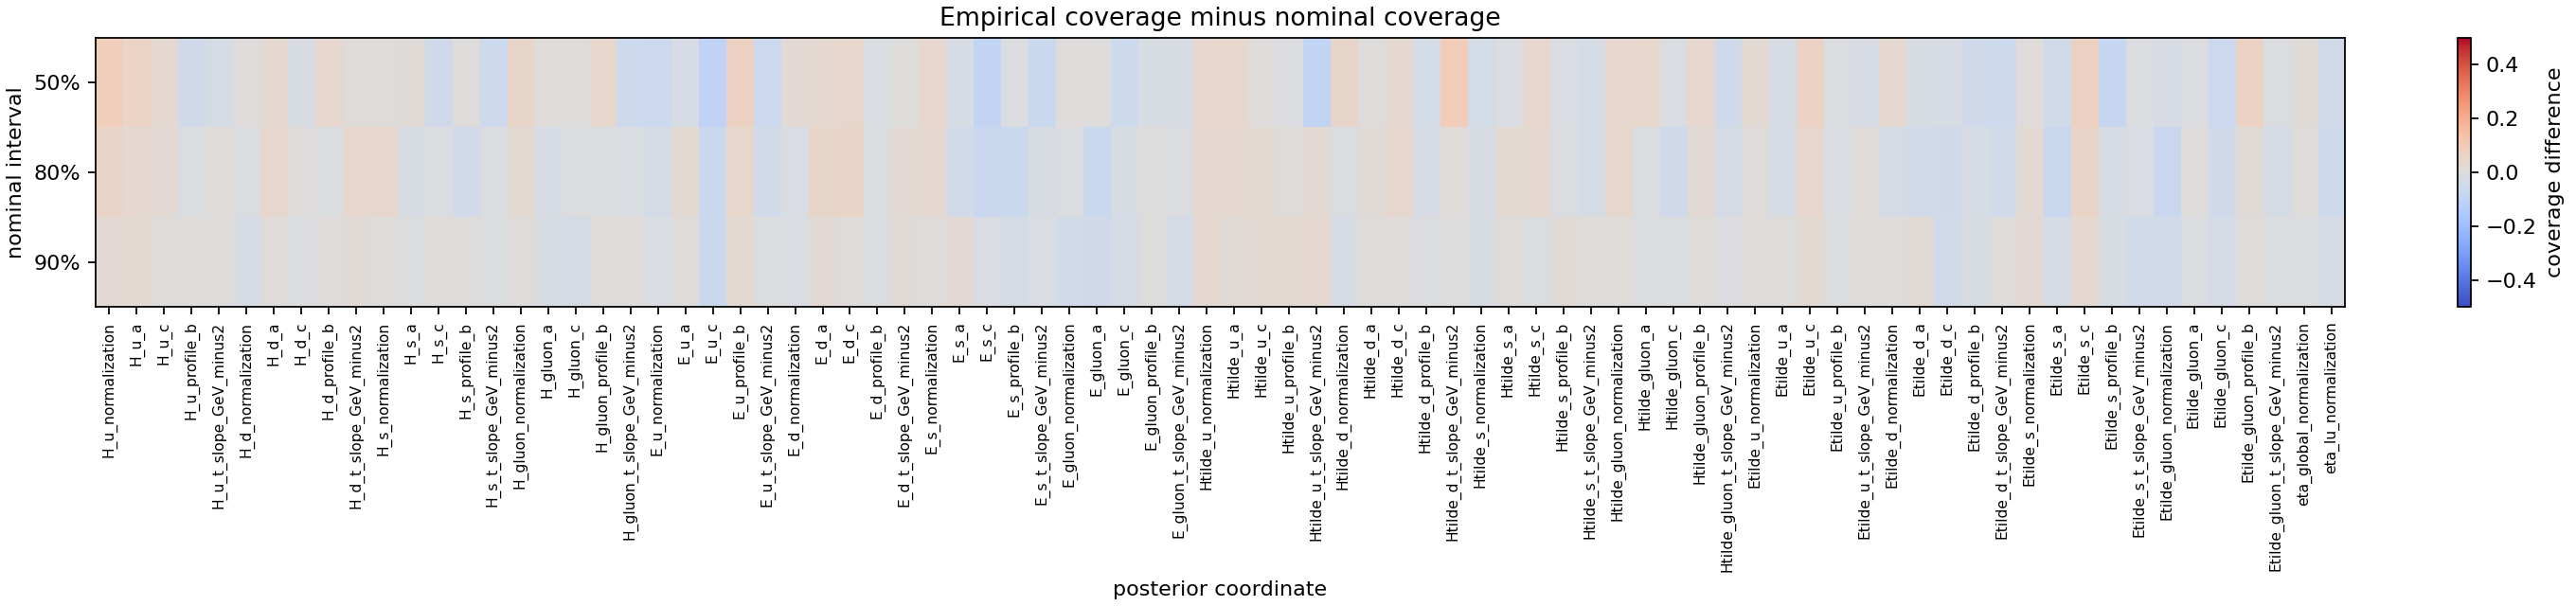
\includegraphics[width=\linewidth,height=.39\textheight,keepaspectratio]{coverage_calibration.png}
\vspace{1mm}
\begin{columns}[T,onlytextwidth]
\column{0.47\textwidth}
\begin{block}{What was tested}
\small
200 independent outer-test truths, 512 posterior samples per trial, and
nominal 50\%, 80\%, and 90\% credible intervals across all 82 posterior
coordinates.
\end{block}
\column{0.50\textwidth}
\begin{block}{Observed result}
\small
Maximum deviation from nominal coverage: \textbf{3.064 standard errors}, below
the frozen 3.5-SE gate. All 64/64 selected posterior physics vectors were valid
under exact-native reevaluation.
\end{block}
\end{columns}
\vspace{2mm}
\small\color{muted}
Coverage asks whether uncertainty is statistically honest over repeated DD-family
problems; it does not establish transfer to another GPD family.
\end{frame}

\begin{frame}{Posterior samples reproduce a withheld synthetic observable set}
\centering
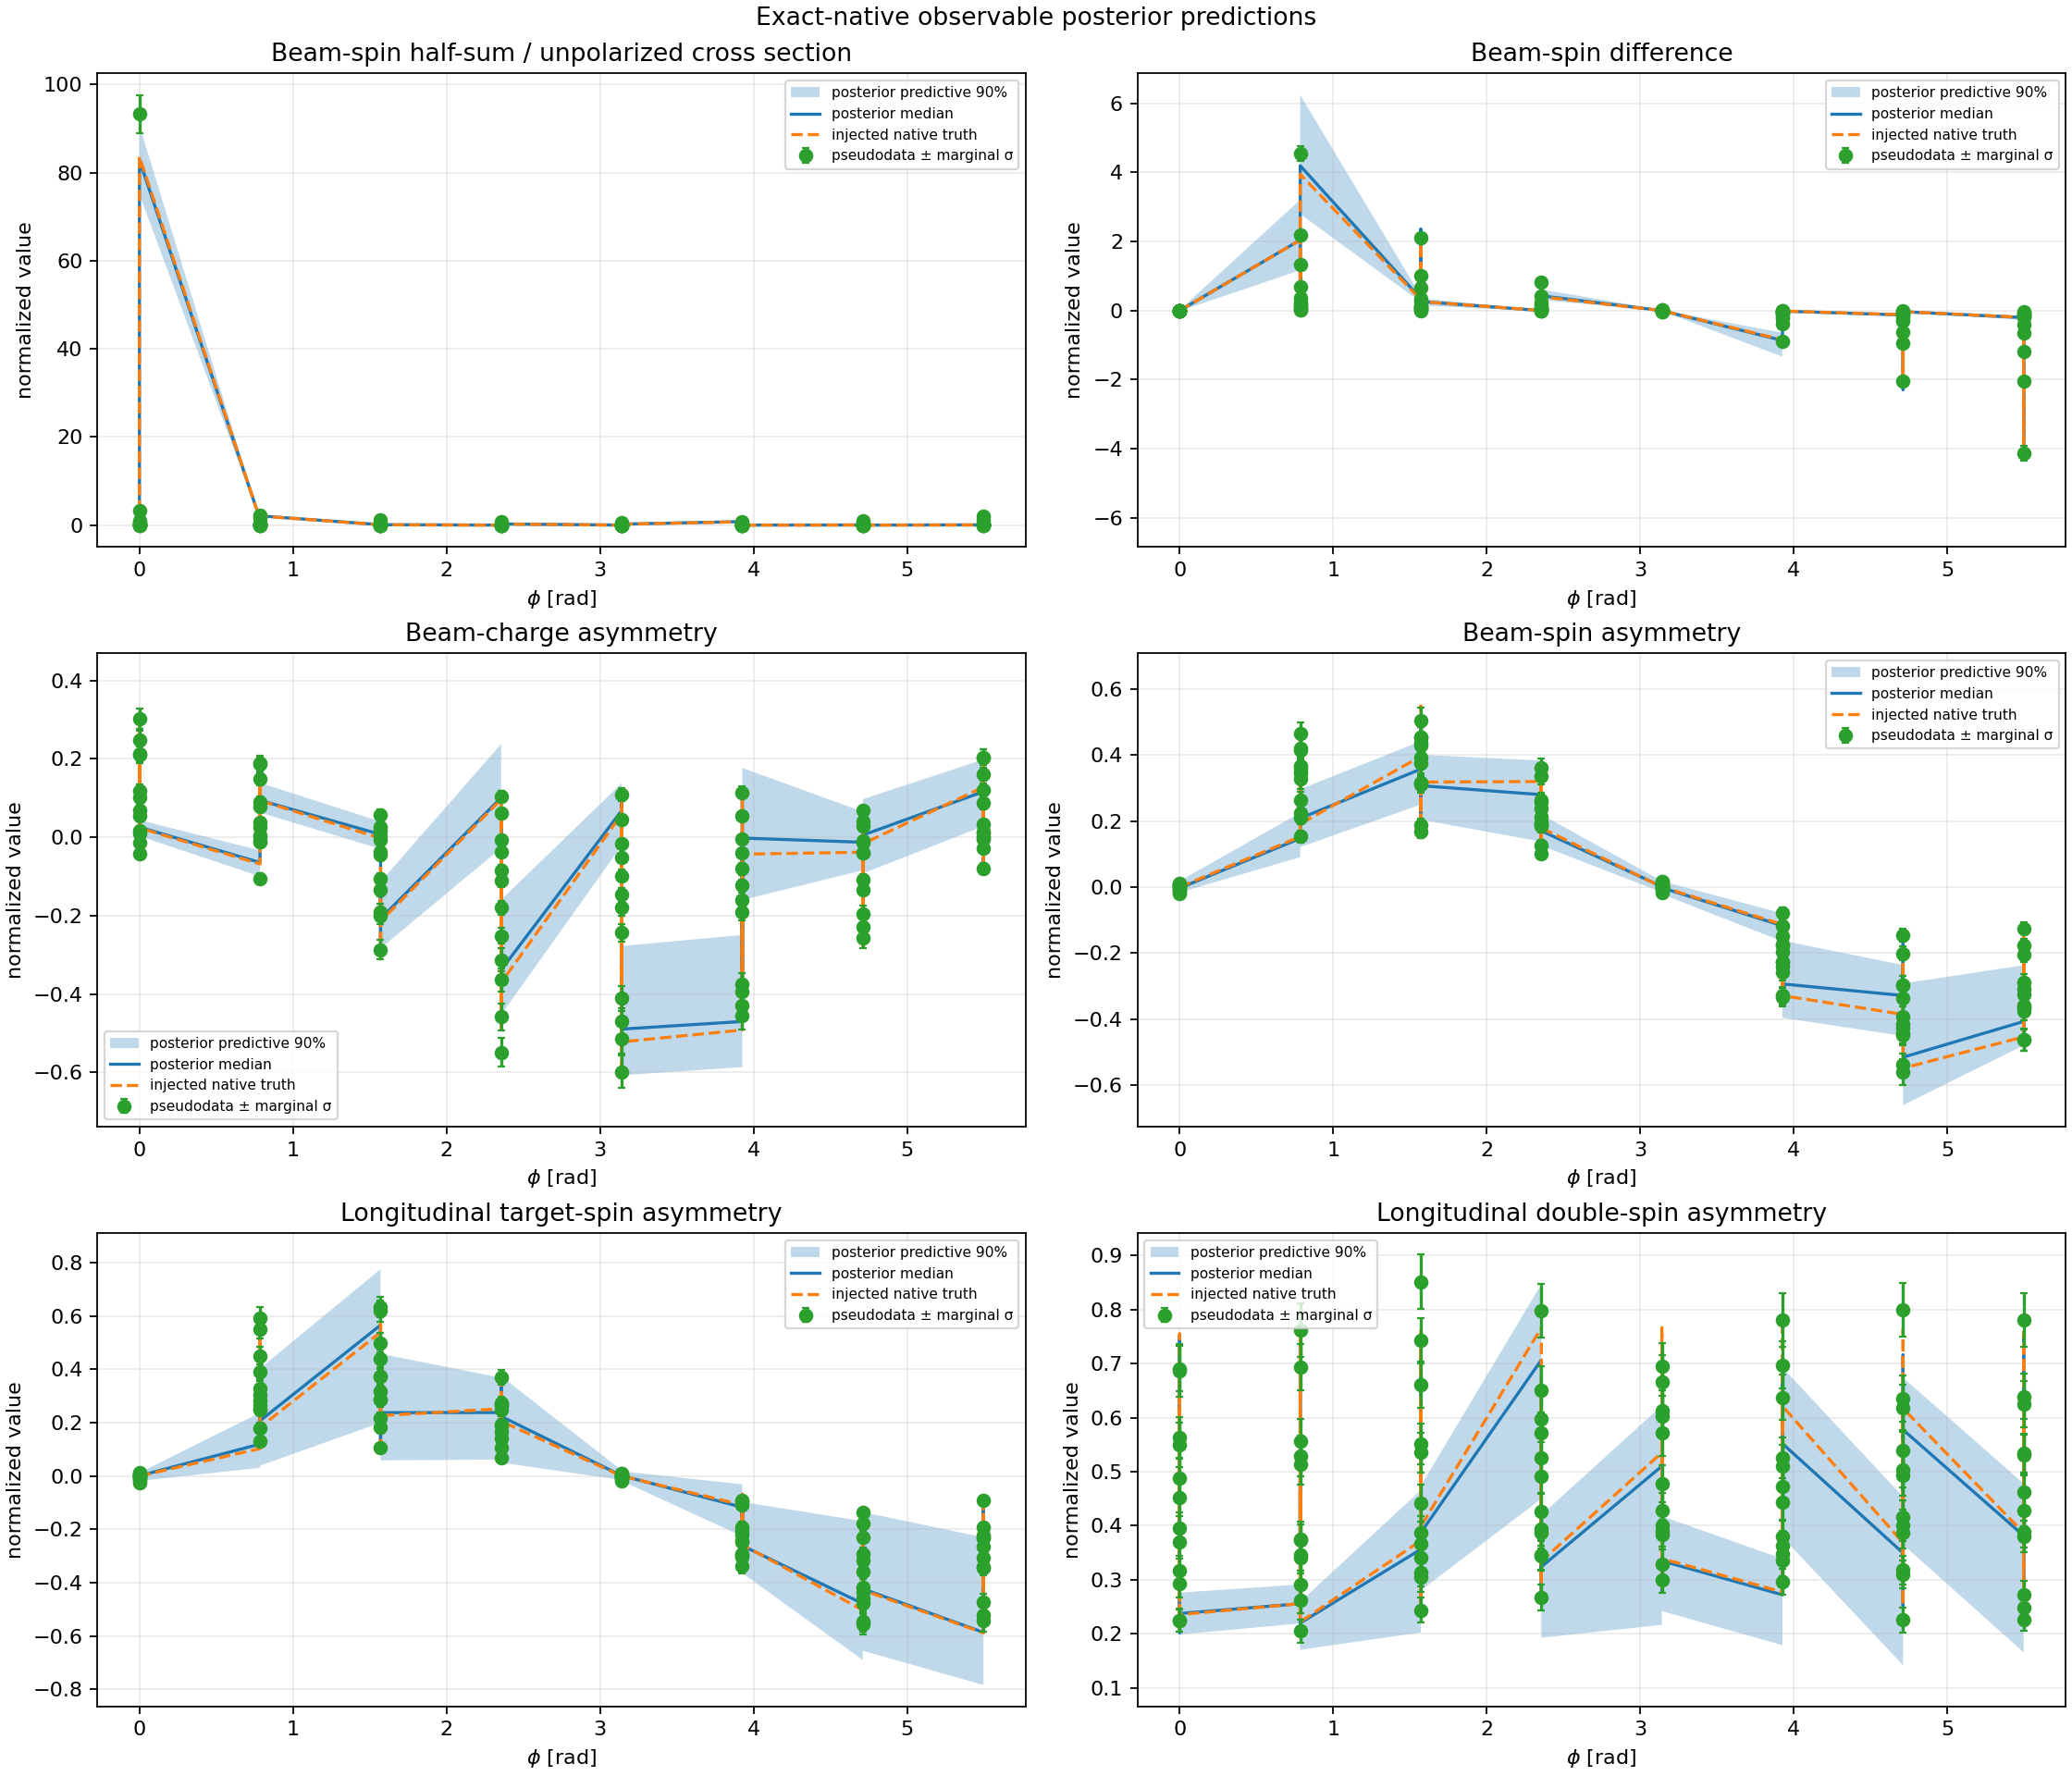
\includegraphics[trim=0 288 0 0,clip,width=.96\linewidth,
  height=.72\textheight,keepaspectratio]{posterior_predictive.png}
\vspace{1mm}
\parbox{.95\linewidth}{\centering\scriptsize\color{muted}
Four representative panels are shown; the stored check includes all six observables.}
\end{frame}

\begin{frame}{A true holdout changes both the physics family and the kinematics}
\begin{columns}[T,onlytextwidth]
\column{0.48\textwidth}
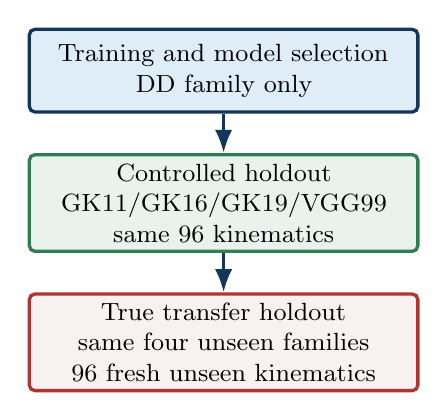
\begin{tikzpicture}[node distance=5mm,font=\small]
  \node[box,text width=4.7cm] (train) {Training and model selection\\DD family only};
  \node[greenbox,text width=4.7cm,below=of train] (same) {Controlled holdout\\GK11/GK16/GK19/VGG99\\same 96 kinematics};
  \node[badbox,text width=4.7cm,below=of same] (fresh) {True transfer holdout\\same four unseen families\\96 fresh unseen kinematics};
  \draw[flow] (train)--(same);
  \draw[flow] (same)--(fresh);
\end{tikzpicture}
\vspace{2mm}
\small Named-model outputs were absent from corpus generation, optimization,
early stopping, and ensemble selection. The frozen network is evaluated once;
the model is not retuned on holdout results.

\column{0.49\textwidth}
\centering
\small Pointwise observable truth coverage by the nominal 90\% bands
\vspace{1mm}
\begin{tabular}{lcc}
\toprule
model & same kinematics & fresh kinematics\\
\midrule
GK11  & 0.806 & 0.759\\
GK16  & 0.859 & 0.780\\
GK19  & 0.797 & 0.747\\
VGG99 & 0.764 & 0.870\\
\bottomrule
\end{tabular}

\vspace{4mm}
\begin{beamercolorbox}[rounded=true,sep=2mm,wd=.93\linewidth]{block body}
\centering\color{red}\bfseries
Both holdout campaigns fail the predeclared predictive-precision gate.
\end{beamercolorbox}
\end{columns}
\end{frame}

\begin{frame}{Fresh-design holdout exposes observable-level bias}
\begin{columns}[T,onlytextwidth]
\column{0.68\textwidth}
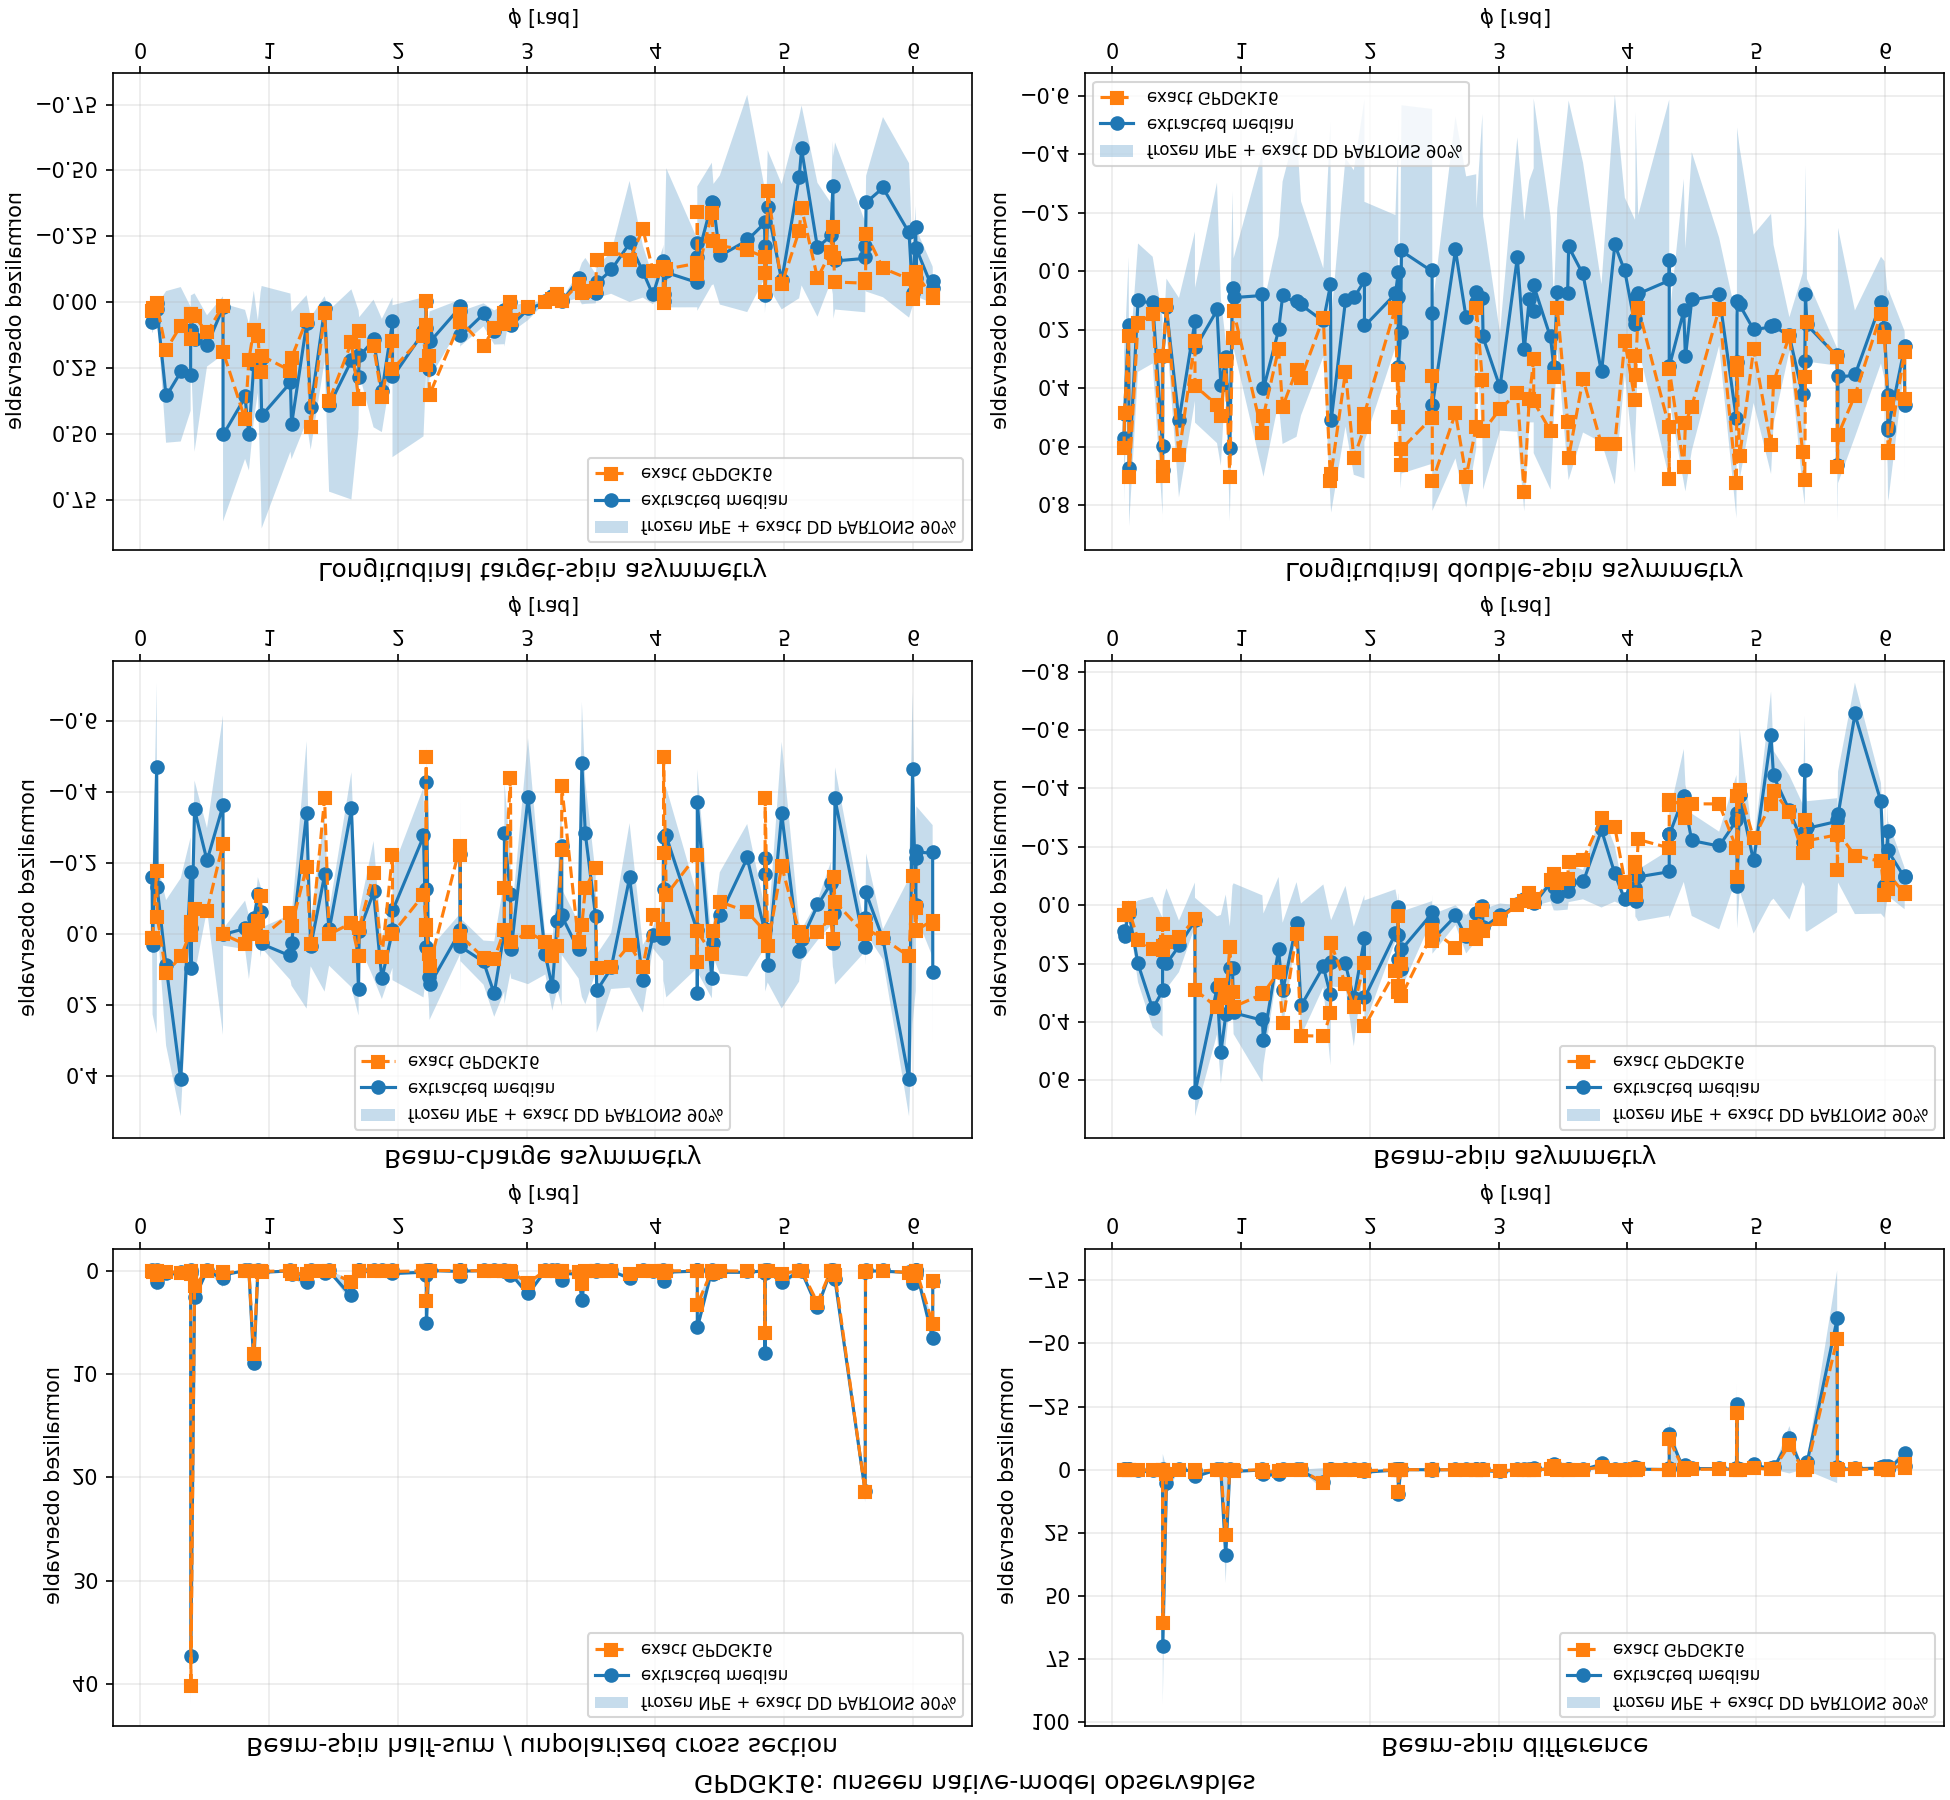
\includegraphics[trim=0 330 0 0,clip,width=\linewidth,
  height=.61\textheight,keepaspectratio]{holdout_plots/holdout-015.png}
\column{0.29\textwidth}
\vspace{2mm}
\textbf{Representative case: GK16}
\vspace{3mm}
\scriptsize
\begin{tabular}{lr}
\toprule
\multicolumn{2}{l}{90\% truth coverage}\\
\midrule
observables & 0.780\\
CFF points & 0.780\\
GPD points & 0.965\\
\bottomrule
\end{tabular}

\vspace{2mm}
\footnotesize
64/64 posterior samples were valid under exact reevaluation, so the mismatch is
scientific rather than an execution failure.

\vspace{2mm}
Broad GPD bands can cover truth while the predicted observables remain biased.
\end{columns}
\takeaway{The current network has learned useful DD-family structure, but not yet a transferable inverse map.}
\end{frame}

\begin{frame}{Representative GPD diagnostic: synthetic closure for $\Huplus$}
\centering
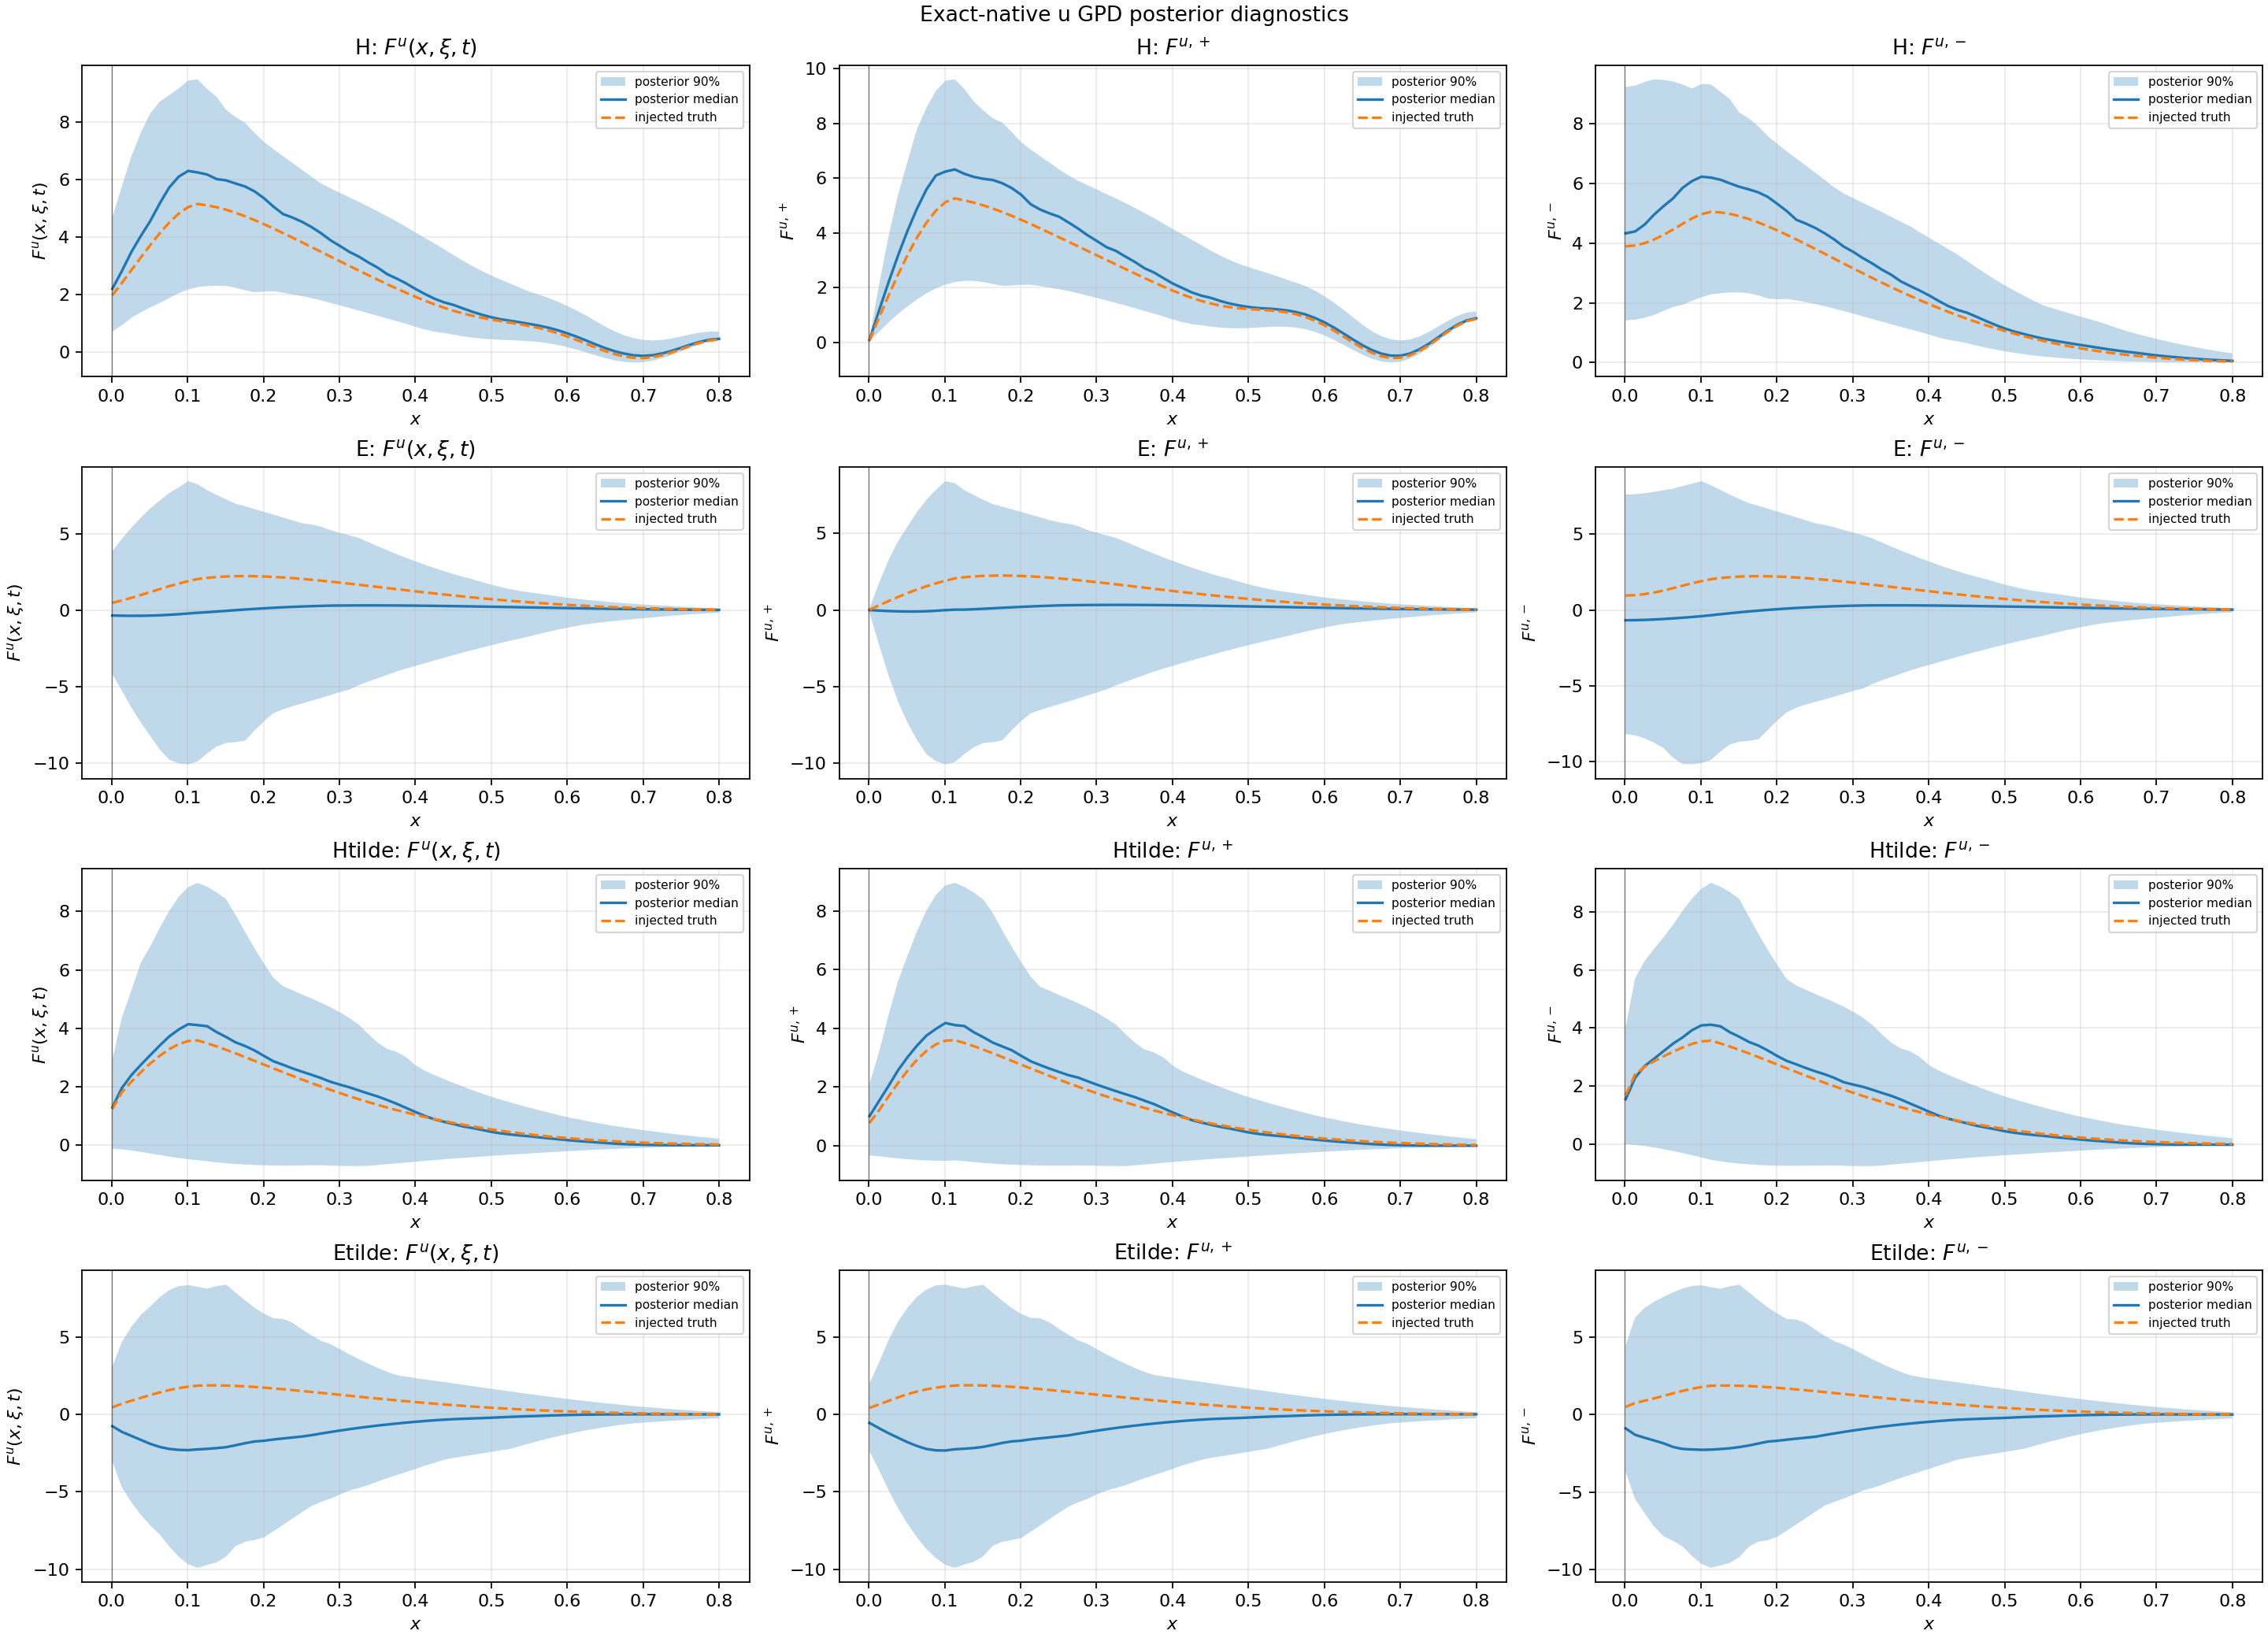
\includegraphics[trim=432 695 432 32,clip,width=.84\linewidth,
  height=.51\textheight,keepaspectratio]{gpd_u_components.png}
\vspace{1mm}
\begin{columns}[T,onlytextwidth]
\column{0.62\textwidth}
\footnotesize Exact PARTONS reevaluation at the declared reference kinematics
$x_B=0.20$, $t=-0.12\,\mathrm{GeV}^2$, $Q^2=2.0\,\mathrm{GeV}^2$.
\column{0.35\textwidth}
\footnotesize\raggedleft Blue band: central 90\% posterior\\
blue line: posterior median\\orange dashed: injected truth
\end{columns}
\takeaway{The median follows the injected C-even shape; uncertainty is largest at low $x$ and honestly retains the truth.}
\end{frame}

\begin{frame}{Representative GPD diagnostic: synthetic closure for $\Huminus$}
\centering
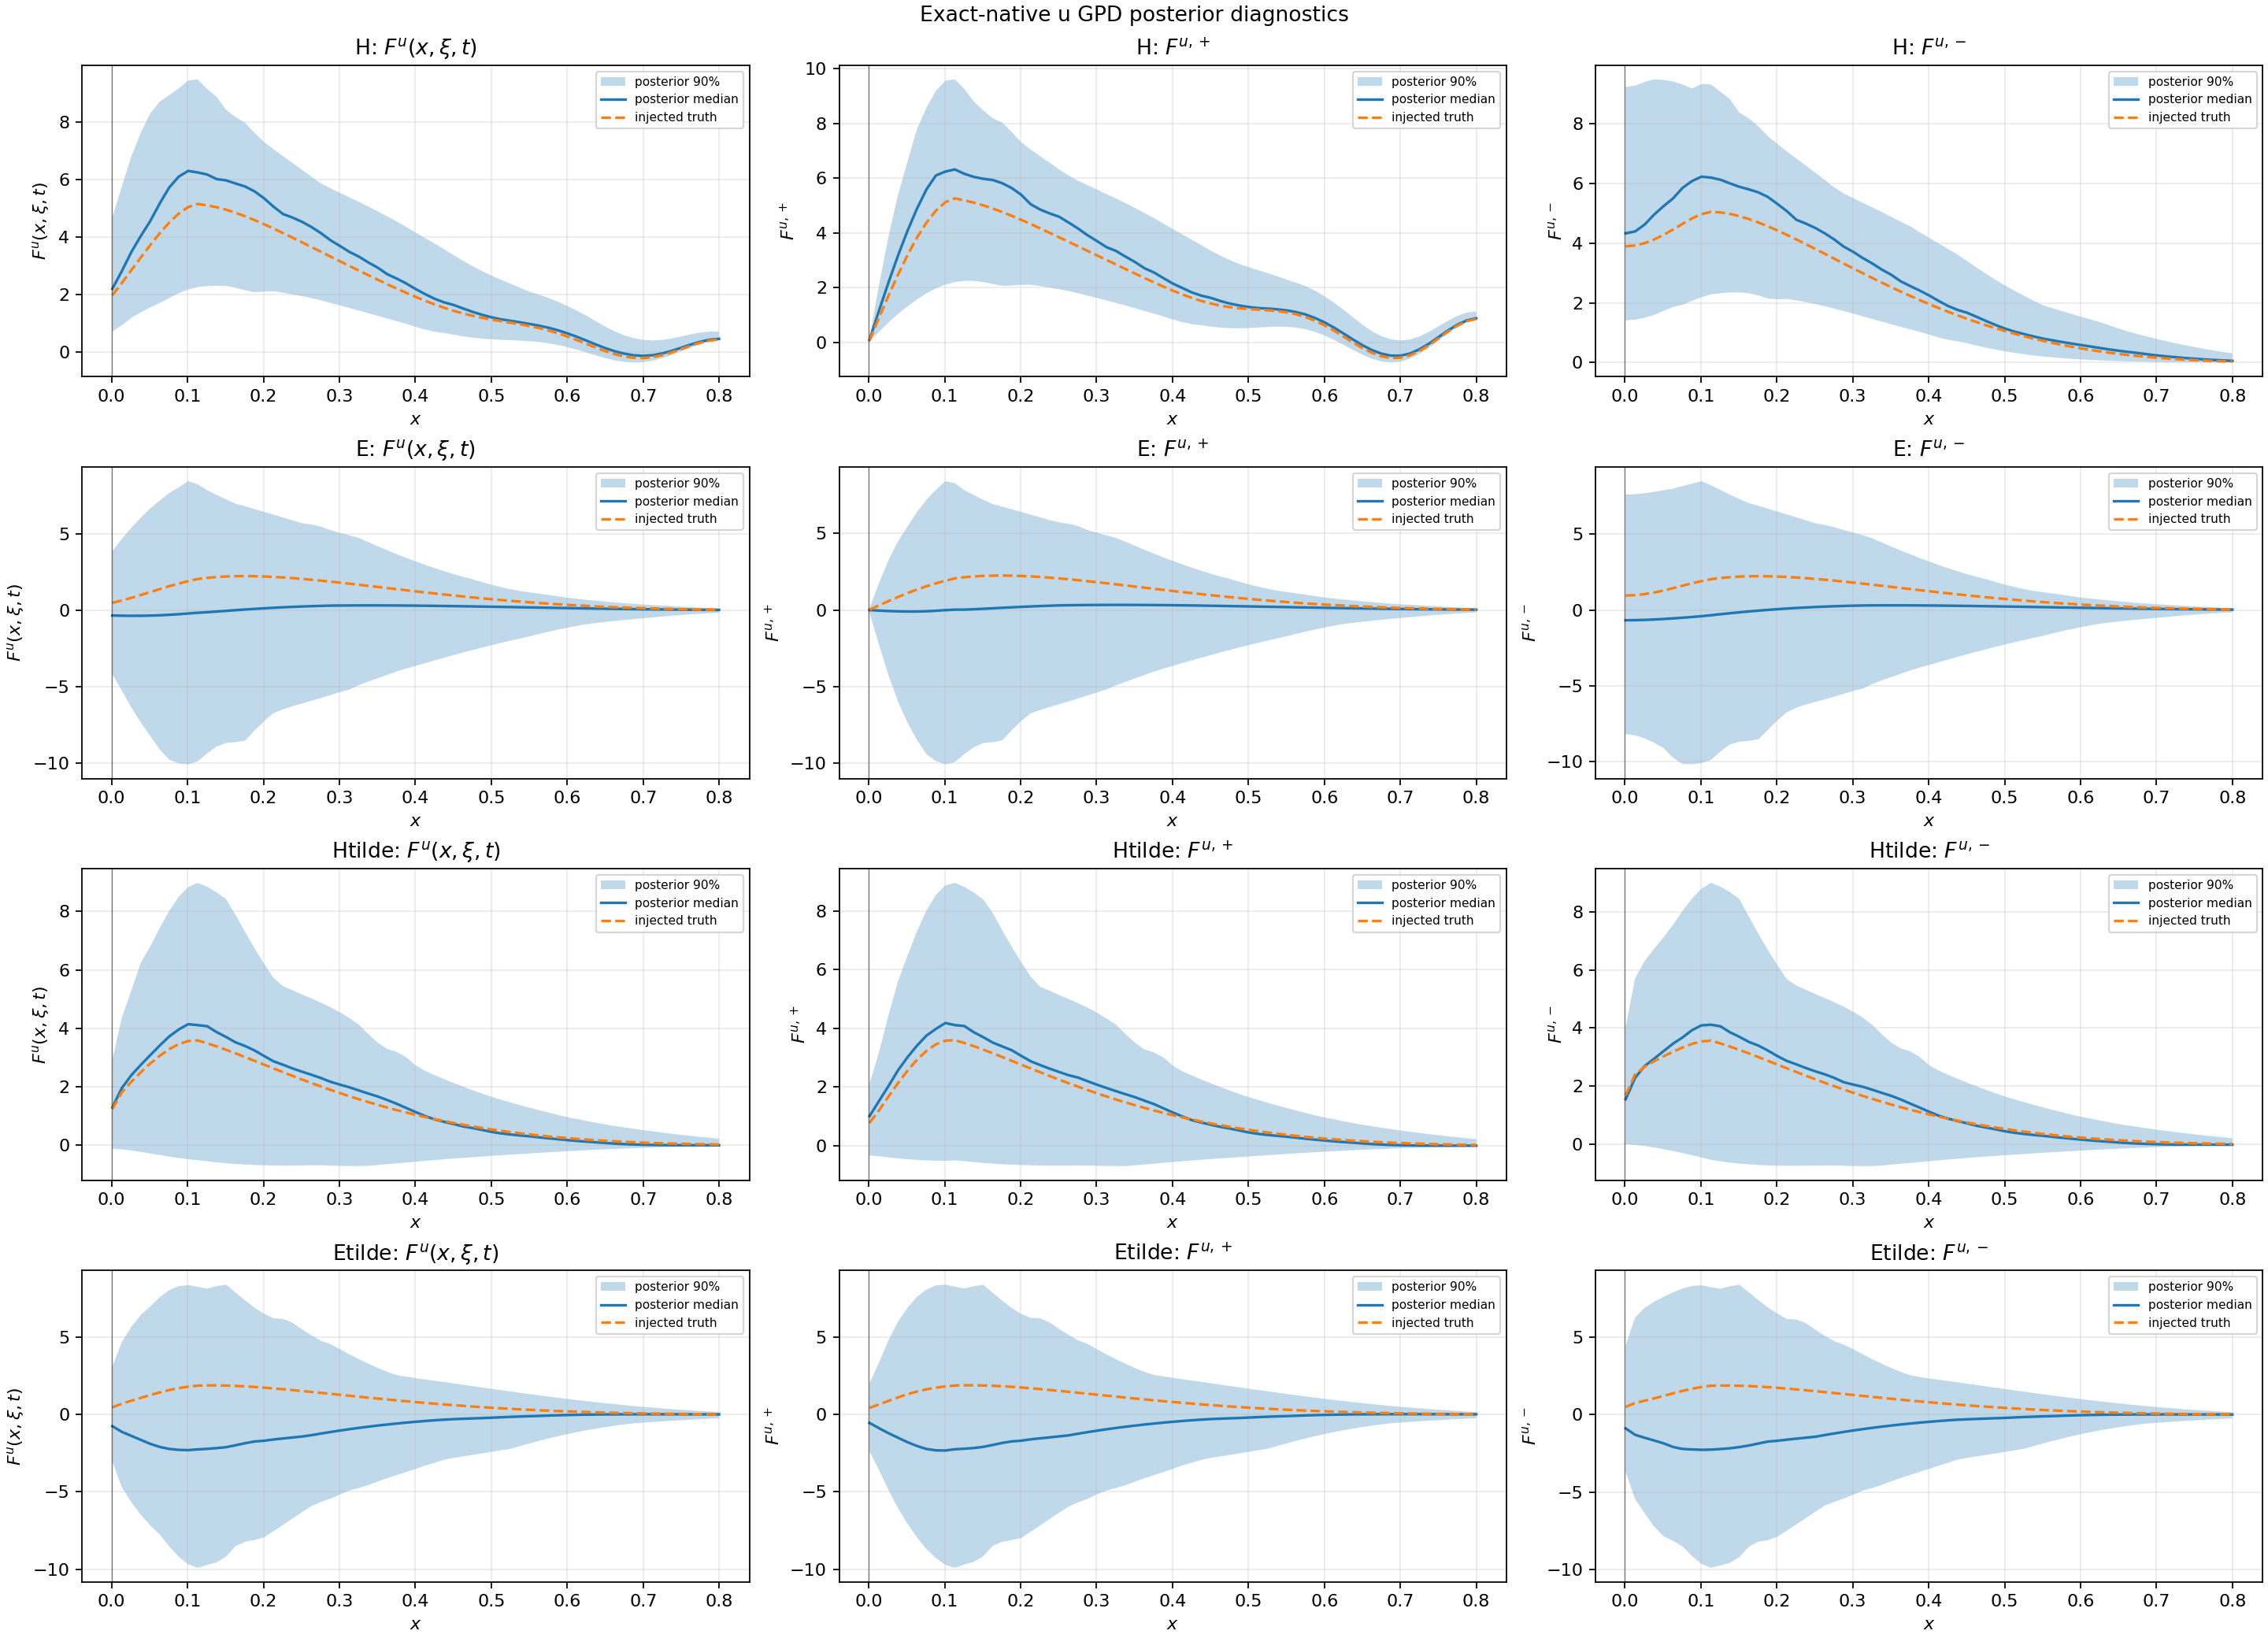
\includegraphics[trim=864 695 4 32,clip,width=.84\linewidth,
  height=.51\textheight,keepaspectratio]{gpd_u_components.png}
\vspace{1mm}
\begin{columns}[T,onlytextwidth]
\column{0.62\textwidth}
\footnotesize Exact PARTONS reevaluation at the same reference kinematics and with the
same posterior samples as the $\Huplus$ panel.
\column{0.35\textwidth}
\footnotesize\raggedleft Blue band: central 90\% posterior\\
blue line: posterior median\\orange dashed: injected truth
\end{columns}
\takeaway{The C-odd/valence-like trend is reproduced, but the low-$x$ band is too broad to claim a precise separation from $\Huplus$.}
\end{frame}

\begin{frame}{What has been demonstrated---and what has not}
\begin{columns}[T,onlytextwidth]
\column{0.48\textwidth}
\begin{block}{Demonstrated}
\begin{itemize}\small\setlength\itemsep{2.5mm}
  \item A DeepSets-conditioned flow learns an 82-dimensional posterior inverse map within the declared DD corpus.
  \item Locked outer-test scores, repeated coverage, posterior predictive checks, and exact reevaluation pass the synthetic gates.
  \item The output spans all modeled $H,E,\widetilde H,\widetilde E$ flavor and gluon sectors; $\Huplus$ and $\Huminus$ provide representative curve-level closure views.
\end{itemize}
\end{block}

\column{0.49\textwidth}
\begin{block}{Current physics limitation}
\begin{itemize}\small\setlength\itemsep{2.5mm}
  \item Fresh GK/VGG families and unseen kinematics expose observable-level bias: nominal 90\% truth coverage is 0.747--0.870.
  \item High holdout GPD coverage is driven partly by broad bands; it is not evidence of precise recovery.
  \item The result is a synthetic closure study, not a real-data extraction. Real-data inference remains disabled.
\end{itemize}
\end{block}
\end{columns}
\takeaway{The next physics challenge is representation robustness: enlarge the training solution space before interpreting any extracted GPD component from data.}
\end{frame}

% The core talk ends above.  The appendix preserves the complete result catalogue
% without forcing dense multi-panel mosaics into the scientific narrative.
\setcounter{framenumber}{0}
\setbeamertemplate{footline}{%
  \leavevmode
  \hbox{%
    \begin{beamercolorbox}[wd=.82\paperwidth,ht=2.6ex,dp=1.1ex,leftskip=.5cm]{author in head/foot}%
      \color{muted}\scriptsize Complete validation catalogue
    \end{beamercolorbox}%
    \begin{beamercolorbox}[wd=.18\paperwidth,ht=2.6ex,dp=1.1ex,rightskip=.45cm plus1fil]{date in head/foot}%
      \color{muted}\scriptsize Appendix \insertframenumber
    \end{beamercolorbox}}
  \vskip0pt}

\begin{frame}[plain]
  \begin{tikzpicture}[remember picture,overlay]
    \fill[navy] (current page.south west) rectangle (current page.north east);
    \draw[orange,line width=3pt]
      ([xshift=2.1cm]current page.south west) --
      ([xshift=2.1cm]current page.north west);
  \end{tikzpicture}
  \vfill
  \hspace{2.25cm}\begin{minipage}{.72\textwidth}
    {\color{white}\LARGE\bfseries Complete validation catalogue\par}
    \vspace{4mm}
    {\color{sky}\large All 19 current training/validation figures and all 24
    controlled- and true-holdout figures\par}
    \vspace{5mm}
    {\color{white}\small One plot per slide preserves labels, bands, and discrepancies
    at projector scale. Appendix numbering is excluded from the 15-slide core talk.\par}
  \end{minipage}
  \vfill
\end{frame}

\begin{frame}{Training history: member-wise train and validation NLL}
\galleryplot{training_validation_nll.png}
\end{frame}

\begin{frame}{Corpus split: grouped train, validation, and outer test}
\galleryplot{dd_train_validation_test_split.png}
\end{frame}

\begin{frame}{Synthetic calibration: empirical credible-interval coverage}
\galleryplot{coverage_calibration.png}
\end{frame}

\begin{frame}{Kinematic support: real catalogue and synthetic pseudodata}
\galleryplot{real_catalog_vs_pseudodata_kinematics.png}
\end{frame}

\begin{frame}{Outer-test posterior predictive distributions}
\galleryplot{posterior_predictive.png}
\end{frame}

\begin{frame}{Outer-test posterior predictive pulls}
\galleryplot{posterior_predictive_pulls.png}
\end{frame}

\begin{frame}{Outer-test CFF real and imaginary components}
\galleryplot{cff_real_imaginary.png}
\end{frame}

\begin{frame}{Outer-test GPD posterior predictions}
\galleryplot{gpd_posterior_predictions.png}
\end{frame}

\begin{frame}{Posterior estimator comparison}
\galleryplot{posterior_comparison.png}
\end{frame}

\begin{frame}{Posterior correlation structure}
\galleryplot{posterior_correlations.png}
\end{frame}

\begin{frame}{Posterior marginals: $H$ sector}
\galleryplot{posterior_marginals_H.png}
\end{frame}

\begin{frame}{Posterior marginals: $E$ sector}
\galleryplot{posterior_marginals_E.png}
\end{frame}

\begin{frame}{Posterior marginals: $\widetilde H$ sector}
\galleryplot{posterior_marginals_Htilde.png}
\end{frame}

\begin{frame}{Posterior marginals: $\widetilde E$ sector}
\galleryplot{posterior_marginals_Etilde.png}
\end{frame}

\begin{frame}{Derived GPD curves: up-quark components}
\galleryplot{gpd_u_components.png}
\end{frame}

\begin{frame}{Derived GPD curves: down-quark components}
\galleryplot{gpd_d_components.png}
\end{frame}

\begin{frame}{Derived GPD curves: strange-quark components}
\galleryplot{gpd_s_components.png}
\end{frame}

\begin{frame}{Derived GPD curves: gluon components}
\galleryplot{gpd_gluon_components.png}
\end{frame}

\begin{frame}{Derived GPD curve: charge-weighted C-even combination}
\galleryplot{gpd_charge_weighted_c_even_sum.png}
\end{frame}

\begin{frame}{Controlled family holdout---GK11 observables}
\holdoutplot{000}
\end{frame}

\begin{frame}{Controlled family holdout---GK11 CFFs}
\holdoutplot{001}
\end{frame}

\begin{frame}{Controlled family holdout---GK11 GPDs}
\holdoutplot{002}
\end{frame}

\begin{frame}{Controlled family holdout---GK16 observables}
\holdoutplot{003}
\end{frame}

\begin{frame}{Controlled family holdout---GK16 CFFs}
\holdoutplot{004}
\end{frame}

\begin{frame}{Controlled family holdout---GK16 GPDs}
\holdoutplot{005}
\end{frame}

\begin{frame}{Controlled family holdout---GK19 observables}
\holdoutplot{006}
\end{frame}

\begin{frame}{Controlled family holdout---GK19 CFFs}
\holdoutplot{007}
\end{frame}

\begin{frame}{Controlled family holdout---GK19 GPDs}
\holdoutplot{008}
\end{frame}

\begin{frame}{Controlled family holdout---VGG99 observables}
\holdoutplot{009}
\end{frame}

\begin{frame}{Controlled family holdout---VGG99 CFFs}
\holdoutplot{010}
\end{frame}

\begin{frame}{Controlled family holdout---VGG99 GPDs}
\holdoutplot{011}
\end{frame}

\begin{frame}{True family + kinematics holdout---GK11 observables}
\holdoutplot{012}
\end{frame}

\begin{frame}{True family + kinematics holdout---GK11 CFFs}
\holdoutplot{013}
\end{frame}

\begin{frame}{True family + kinematics holdout---GK11 GPDs}
\holdoutplot{014}
\end{frame}

\begin{frame}{True family + kinematics holdout---GK16 observables}
\holdoutplot{015}
\end{frame}

\begin{frame}{True family + kinematics holdout---GK16 CFFs}
\holdoutplot{016}
\end{frame}

\begin{frame}{True family + kinematics holdout---GK16 GPDs}
\holdoutplot{017}
\end{frame}

\begin{frame}{True family + kinematics holdout---GK19 observables}
\holdoutplot{018}
\end{frame}

\begin{frame}{True family + kinematics holdout---GK19 CFFs}
\holdoutplot{019}
\end{frame}

\begin{frame}{True family + kinematics holdout---GK19 GPDs}
\holdoutplot{020}
\end{frame}

\begin{frame}{True family + kinematics holdout---VGG99 observables}
\holdoutplot{021}
\end{frame}

\begin{frame}{True family + kinematics holdout---VGG99 CFFs}
\holdoutplot{022}
\end{frame}

\begin{frame}{True family + kinematics holdout---VGG99 GPDs}
\holdoutplot{023}
\end{frame}

\end{document}
